
\chapter{Waves on a Sloping Beach; Shallow Water Theory}\label{chap5}

IN\pageoriginale THE LAST chapter we considered flow over a horizontal level surface. In the case of a non-uniform bottom, we will get an additional term in the horizontal momentum equation due to the force acting on the bottom surface.

\section{Shallow water equations}\label{chap5:sec5.1}

We choose a coordinate system $x,y$ such that $y=-h_0(x)$ denotes the bottom and $y=\eta(x,t)$ the water surface. Hence the total depth $h(x,t)$ is 
$$
h(x,t)=h_0(x)+\eta(x,t).
$$

The equation of conservation of mass is 
\begin{equation}
\frac{d}{dt}\int\limits_{x_2}^{x_1}h(x,t)\,dx+[uh]_{x_2}^{x_1}=0 \tag{5.1}\label{chap5:eq5.1}
\end{equation}
as before, and if $u$ and $h$ are continuously differentiable, then 
\begin{equation}
h_t+(uh)_x=0.\tag*{$(5.1)'$}\label{chap5:eq5.1'}
\end{equation}
\begin{figure}[H]
\centering
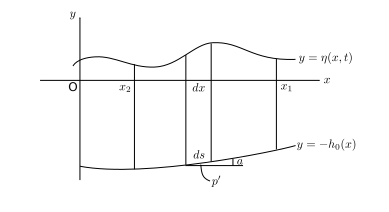
\includegraphics{figures/fig61-5.1.eps}
\caption{}
\label{chap1:fig5.1}
\end{figure}


Let\pageoriginale us now consider the momentum balance in the $x$-direction. Let $p'$ be the excess pressure as before. When the bottom is not horizontal, the contribution of $p'$ from the bottom surface will have a non-zero horizontal component. Let us consider a thin section of thickness $dx$ and let $ds$ be the line element along the bottom $y=-h_0(x)$. Let $\alpha$ be the inclination of $ds$ to the $x$-axis. Then 
$$
ds=\frac{dx}{\cos\alpha}.
$$

Hence the momentum balance in the horizontal direction is 
\begin{equation}
\frac{d}{dt}\int\limits_{x_2}^{x_1}\,hu\,dx+\left[hu^2+\frac{1}{2}\,gh^2 \right]_{x_2}^{x_1}= -\int\limits_{x_2}^{x_1}\left(p'\frac{dx}{\cos\alpha}\right) \sin\alpha\tag{5.2}\label{chap5:eq5.2}
\end{equation}
In the shallow water theory we have $p'=g(\eta-y)$. At $y=-h_0, p'=g(\eta+h_0)=gh$. Therefore \eqref{chap5:eq5.2} becomes 
\begin{equation}
\frac{d}{dt}\int\limits_{x_2}^{x_1}\,hu\,dx+\left[hu^2+\frac{1}{2}\,gh^2 \right]_{x_2}^{x_1}=\int\limits_{x_2}^{x_1}\,gh\frac{dh_0}{dx}\,dx, \tag{5.3}\label{chap5:eq5.3}
\end{equation}
since $\frac{dh_0}{dx}=\tan\alpha$. If all the quantities are smooth, in the limit $x_2\to x_1$, we obtain
\begin{equation}
(hu)_t+\left(hu^2+\frac{1}{2}\,gh^2\right)_x=gh\frac{dh_0}{dx} \tag{5.4}\label{chap5:eq5.4}
\end{equation}

When there are discontinuities, the shock condition derived from \eqref{chap5:eq5.3} is 
$$
-U[hu]+\left[hu^2+\frac{1}{2}\,gh^2\right]=0,
$$
since the right hand side of \eqref{chap5:eq5.3} becomes zero in the limit $x_2\to x_1$. Thus, the shock conditions are unaffected by the extra term $gh\frac{dh_0}{dx}$ due to the non-uniform bottom. 

Using\pageoriginale the mass conservation equation \ref{chap5:eq5.1'} the momentum equation \eqref{chap5:eq5.4} can be written as 
$$
u_t+uu_x+g\eta_x=0.
$$

Hence the system of equations for the flow of shallow water over a non-uniform bottom is 
\begin{equation}
\left.
\begin{aligned}
& h_t+uh_x+hu_x = 0,\\
& u_t+uu_x+g\eta_x =0,\\
& h=h_0+\eta.
\end{aligned}
\right\}\tag{5.5}\label{chap5:eq5.5}
\end{equation}

\section{Linearized equations}\label{chap5:sec5.2}

We assume that the disturbances are small of order $\epsilon \ll 1$ \ie $\frac{\eta}{h_0}=0(\epsilon)$ and $\frac{u}{\sqrt{gh_0}}=o(\epsilon)$. We also assume that the derivative are also of the same order.

Since $h=\eta(x,t)+h_0(x)$, equations \eqref{chap5:eq5.5} can be written down as 
\begin{align}
\eta_t &+ uh'_0+h_0u_x+u\eta_x+\eta u_x=0\tag{5.6}\label{chap5:eq5.6}\\
u_t &+ uu_x+g\eta_x=0.\tag{5.7}\label{chap5:eq5.7}
\end{align}

The first three terms of \eqref{chap5:eq5.6} are of order $0(\epsilon)$ whereas the last two terms are of order $0(\epsilon^2)$. In the equation \eqref{chap5:eq5.7} $uu_x=0(\epsilon^2)$ and the other terms are of order $\epsilon$. Hence to a first order approximation we have 
\begin{equation}
\left.
\begin{aligned}
\eta_t &+ h_0u_x+h'_0u=0,\\
u_t &+ g\eta_x=0.
\end{aligned}
\right\}\tag{5.8}\label{chap5:eq5.8}
\end{equation}

Equations \eqref{chap5:eq5.8} are the linearized versions of equations \eqref{chap5:eq5.5}. Differentiating\pageoriginale the first equation of \eqref{chap5:eq5.8} partially w.r.t. $t$ and using the second equation, we obtain
\begin{equation}
\eta_{tt}=gh_0\eta_{xx}+gh'_0\eta_x.\tag{5.9}\label{chap5:eq5.9}
\end{equation}

This is the wave equation with an additional term. If $h_0$ were constant then 
$$
\eta_{tt}=gh_0\eta_{xx}
$$
and the general solution of this is 
$$
\eta=f_1\left(x-\sqrt{gh_0}t\right)+f_2\left(x-\sqrt{gh_0}t\right).
$$

The velocity of propagation is $\sqrt{gh_0}$. 

\section{Linear theory for waves on a sloping beach}\label{chap5:sec5.3}

We now consider a sloping beach with inclination $\beta$ to the horizontal. We assume $\beta$ to be small so that linearized shallow water theory can be applied.

However there will be some questions about validity to be considered later. These are 
\begin{enumerate}
\item [(i)] The question of using the shallow water theory as $x\to\infty$, when the water becomes deep. 
\item [(ii)] The question of the assumption $\eta/h_0\ll 1$ near $x=0$ where $h_0\to 0$.
\end{enumerate}

We have to solve equation \eqref{chap5:eq5.9} with $h_0=x\tan\beta$ and we take $h_0\simeq\beta x$ since $\beta$ is very small. Hence the equation can be written as 
\begin{equation}
\eta_{tt}=g\beta x\eta_{xx}+g\beta\eta_x.\tag{5.10}\label{chap5:eq5.10}
\end{equation}

Let $\eta=N(x)e^{-i\omega t}$ be a solution of equation \eqref{chap5:eq5.10}. Then we obtain\pageoriginale an ordinary differential equation for $N$ as follows:
\begin{equation}
N''+\frac{1}{x}N'+\frac{\omega^2}{g\beta}\;\frac{1}{x}N=0. \tag{5.11}\label{chap5:eq5.11}
\end{equation}

This is to be solved in $0< x <\infty$.

The point $x=0$ is a regular point of equation \eqref{chap5:eq5.11}, and $x=\infty$ is an irregular point. This suggests a transformation to Bessel's equation or some other confluent hypergeometric equation. In fact the transformation 
$$
x=\frac{g\beta}{\omega^2}\;\frac{X^2}{4}
$$
converts it into the Bessel equation of order zero.
\begin{equation}
\frac{d^2N}{dX^2}+\frac{l}{X}\;\frac{dN}{dX}+N=0.\tag{5.12}\label{chap5:eq5.12}
\end{equation}

The Bessel functions $J_0(X), Y_0(X)$ are two linearly independent solutions of the equation \eqref{chap5:eq5.12}. Hence a general solution of \eqref{chap5:eq5.11} is 
$$
N=AJ_0\left(2\omega \sqrt{\frac{x}{g\beta}}\right)-iBY_0\left(2\omega  \sqrt{\frac{x}{g\beta}}\right),
$$
where $A$ and $B$ are constants. Since the power series for $J_0(X)$ contains only even powers of $X$, $J_0 \left(2\omega \sqrt{\frac{x}{g\beta}} \right)$ is an integer power series in $x$ and is regular at the beach $x=0$. We note that $Y_0$ has a logarithmic singularity at $x=0$. 

The complete solution of \eqref{chap5:eq5.10} is 
$$
\eta(x,t)=\left\{AJ_0\left(2\omega \sqrt{\frac{x}{g\beta}}\right)-iBY_0 \left(2\omega \sqrt{\frac{x}{g\beta}}\right)\right\}e^{-i\omega t}.
$$

As $x\to\infty$ the asymptotic formula for $\eta$ is 
\begin{equation}
\begin{aligned}
\eta &\sim\frac{1}{\sqrt{\pi}}\left(\frac{g\beta}{\omega^2 x}\right)^{1/4} \frac{A+B}{2}\exp\left(-i2\omega \sqrt{\frac{x}{g\beta}}-i\omega t+\frac{\pi i}{4}\right)\\
&+ \frac{A-B}{2}\exp\left(i2\omega \sqrt{\frac{x}{g\beta}}-i\omega t-\frac{\pi i}{4}\right).
\end{aligned}\tag{5.13}\label{chap5:eq5.13}
\end{equation}\pageoriginale

The first term in the bracket corresponds to an incoming wave and the second one to an outgoing wave. In a uniform medium an outgoing periodic wave is given by 
$$
ae^{i\kappa x-i\omega t},
$$
where $\kappa, \omega, a$ are the wave number, frequency and amplitude respectively. The terms in \eqref{chap5:eq5.13} are generalizations to the form 
$$
a(x,t)e^{i\theta(x,t)}.
$$

A generalized wave number and frequency can be defined in terms of the phase function $\theta(x,t)$ by 
\begin{equation}
\kappa(x,t)=\theta_x,\; \nu(x,t)= -\theta_t;\tag{5.14}\label{chap5:eq5.14}
\end{equation}
the generalized phase velocity is 
\begin{equation}
c(x,t)=\frac{\nu}{k}= -\frac{\theta_t}{\theta_x}.\tag{5.15}\label{chap5:eq5.15}
\end{equation}

The function $a(x,t)$ is the amplitude.

In our particular case the outgoing wave has 
$$
\theta(x,t)=2\omega \sqrt{\frac{x}{g\beta}}-\omega t-\frac{\pi}{4}.
$$

Hence the wave number, frequency and phase velocity are 
\begin{align*}
\kappa(x,t) &=\theta_x=\frac{\omega}{\sqrt{g\beta x}},\\
\nu(x,t) &= -\theta_t=\omega,\\
c(x,t) &= \sqrt{g\beta x}.
\end{align*}

We note that the waves get shorter as $x\to 0$, and that $c=\sqrt{gh_0(x)}$ is\pageoriginale the generalization of the result for constant depth. The incoming wave is similar with the opposite sign of propagation.
\medskip

\subsection*{\bf Behavior as $x\to\infty$}.

We note that the amplitude a varies proportional to $x^{-1/4}$. As $x\to\infty, a\to 0$. This means that, within shallow water, we cannot pose the natural problem of a prescribed incoming wave at infinity with a given {\bf nonzero} amplitude. This is due to the failure of the shallow water assumptions at $\infty$, one of the questions noted at the beginning of this section. It it found from the full theory in Chapter \ref{chap7}, (for the solution corresponding to $J_0$) that the ratio of amplitude at infinity $a_\infty$ to amplitude at shoreline $a_0$ is in fact $(2\beta/\pi)^{1/2}$. Therefore, $a_\infty/a_0\to 0$ as $\beta\to 0$, and the $x^{-1/4}$ behavior is the shallow water theory's somewhat inadequate attempt to cope with this. However, the full solution does show that the shallow water theory is a good approximation near the shore. And it is valuable there since, for example, the corresponding nonlinear solution can be found in the shallow water theory (see the next section) but not in the full theory.

\subsection*{\bf Behavior as $x\to 0$ and breaking}.

We see from \eqref{chap5:eq5.13} that the ratio of $B$ to $A$, which controls the amount of $J_0$ and $Y_0$ in the solution, also determines the proportion of incoming wave that is reflected back to infinity. 

For\pageoriginale $B=0$, we have perfect reflection with
\begin{equation}
\eta=AJ_0\left(2\omega\frac{\sqrt{x}}{g\beta}\right)e^{-i\omega t} \tag{5.16}\label{chap5:eq5.16}
\end{equation}
and the solution is bounded and regular at the shoreline $x=0$.

In the other extreme, $A=B$, there is no reflection, we have a purely incoming wave
\begin{equation}
\eta=A\left(J_0-iY_0\right)e^{-i\omega t},\tag{5.17}\label{chap5:eq5.17}
\end{equation}
but it is now singular at the shoreline. The interpretation of the singularity is that it is the linear theory's crude attempt to represent the breaking of waves and the associated loss of energy. As $B$ increases, more energy goes into the singularity (breaking) and less is reflected. 

Although breaking is the most obvious phenomenon we observe at the seashore, a number of long wave phenomena (long swells, edge waves, tsunamis) are in the range where breaking does not occur so that the $J_0$ solution $(B=0)$ with perfect reflection is relevant. This is fortunate since practical use of the $Y_0$ solution would be limited, although the situation is mathematically interesting.

The singular solution is related also to the second question noted at the beginning of this section: The breakdown of the linearizing assumption $\eta/h_0\ll 1$ as $h_0\to 0$ at the shoreline. On this we can say that the nonlinear solution corresponding to $J_0$ can be found without this assumption (next section), and it endorses the linear approximation. The $Y_0$ solution with its crucial ties to\pageoriginale complicated nonlinear breaking is clearly a different matter.

\subsection*{\bf The eigenvalue problem and expansion theorem}. 

One further aspect of the $Y_0$ solution is certainly intriguing mathematically. The eigenvalue problem \eqref{chap5:eq5.11} with $\omega^2/g\beta$ as eigenparameter is of ``limit circle'' type at $x=0$. This is identified by the fact that {\bf both} solutions are square integrable there and it has important remifications in the general theory of eigenfunction expansions. The main one is that various choices of linear combinations of $J_0$ and $Y_0$ each lead to a satisfactory eigenfunction expansion to represent a given square integrable function (as required, say, in solving the initial value problem). In our context this is interpreted as an arbitrary choice of the degree of breaking, within this theory. The natural choice would then appear to be an expansion theorem
\begin{equation}
f(x)=\int\limits_0^\infty A(\omega)\left\{J_0\left(2\omega \sqrt{\frac{x} {g\beta}}\right)-imY_0\left(2\omega \sqrt{\frac{x}{g\beta}}\right)\right\}\, d\omega\tag{5.18}\label{chap5:eq5.18}
\end{equation}
where {\bf we must give $m$} in the range $0\leq m\leq 1$ to indicate our estimate of the relative amount of breaking. With the choice $m=0$ this is the usual Fourier-Bessel expansion, and is certainly one valid possibility. When $m\neq 0$, the result obtainde from the usual general theory (see Titchmarsh \cite{key2}, p.~78) is not quite \eqref{chap5:eq5.18}. The $Y_0$ has to be replaced by 
\begin{equation}
Y_0\left(2\omega \sqrt{\frac{x}{g\beta}} \; \right)-\frac{2}{\pi}J_0\left(2\omega \sqrt{\frac{x}{g\beta} } \; \right)\log\omega.\tag{5.19}\label{chap5:eq5.19}
\end{equation}\pageoriginale

It seems hard to find a ``natural'' physical interpretation for this modification. Moreover, one may still ask whether the unmodified form \eqref{chap5:eq5.18} is in fact a correct possible choice. A further question that arises, since we expect different amounts of breaking for different frequencies, is whether there is an expansion theorem for reasonable choices of {\bf functions} $m(\omega)$ in \eqref{chap5:eq5.18}.

It might be remarked that these points are particularly interesting because in most applications where the ``limit circle'' case arises, only a bounded solution makes physical sense and the one parameter arbitrariness is not in fact used in any significant way. The niceties of the mathematical discussion are not displayed.

\subsection*{\bf Tidal estuary problem}.

In a channel where the breadth $b(x)$ varies, as well as the depth $h_0(x)$, the shallow water equations are modified to 
\begin{align*}
\frac{\partial}{\partial t}\left\{\left(h_0+\eta\right)b\right\}&+ \frac{\partial}{\partial x}\left\{\left(h_0+\eta\right)ub\right\}=0,\\
\frac{\partial u}{\partial t}+u\frac{\partial u}{\partial x}+g\frac{\partial\eta}{\partial x} &=0.
\end{align*}

For the case $h_0(x)=\beta x, b(x)=\alpha x$ the linearized equation for $\eta$ can again be solved in Bessel functions. G.I. Taylor used this solution to study the large tidal variations in the Bristol channel. In this application to extremely long waves, breaking is not an issue and only the $J_n$ solution is accepted.

\section{Nonlinear waves on a sloping beach}\label{chap5:sec5.4}\pageoriginale 

In Section \ref{chap5:sec5.3} we considered the linear approximation of the equations for waves on a sloping beach. Carrier and Greenspan \cite{key4} in 1958 gave an exact solution of the nonlinear equations using a modified type of hodograph transformation applied to characteristic variables. We recall that the governing equations are 
\begin{align*}
h_t &+ uh_x+hu_x=0,\\
u_t &+ uu_x+gh_x-g\beta =0,
\end{align*}
where $h=\beta x+\eta(x,t)$. 

Introducing the variable $c=\sqrt{gh}$, which we know to be significant, the above equations become
\begin{equation}
\left.
\begin{aligned}
& 2c_t+2uc_x+cu_x=0,\\
& u_t+uu_x+2cc_x-g\beta=0.
\end{aligned}
\right\}\tag{5.20}\label{chap5:eq5.20}
\end{equation}

Due to the presence of the term $g\beta$, the straight forward hodograph transformation $(u,c)\to(x,t)$ will not simplify the equations, since this time the Jacobian $\mathfrak{g}$ would not cancel through. However, Carrier and Greenspan introduced new variables suggested by the characteristic forms and applied a hodograph transformation to these.

The characteristic forms of the equations \eqref{chap5:eq5.20} are 
\begin{align*}
(u+2c)_t &+ (u+c)\;(u+2c)_x -g\beta =0,\\
(u-2c)_t &+ (u-c)\;(u-2c)_x -g\beta =0.
\end{align*}
 These\pageoriginale can be written as
\begin{align*}
(u+2c-g\beta t)_t &+ (u+c)\;(u+2c-g\beta t)_x=0,\\
(u-2c-g\beta t)_t &+ (u-c)\;(u-2c-g\beta t)_x=0.
\end{align*}

The $\mathscr{C}_+$ and $\mathscr{C}_-$ characteristic curves are defined by 
\begin{equation}
\left.
\begin{aligned}
\mathscr{C}_+:\frac{dx}{dt} &= u+c, \; u+2c-g\beta t=\text{constant},\\
\mathscr{C}_-:\frac{dx}{dt} &= u-c, \; u-2c-g\beta t=\text{constant}.
\end{aligned}
\right\}\tag{5.21}\label{chap5:eq5.21}
\end{equation}

We define the characteristic variables $p,q$ by 
\begin{align}
p &= u+2c-g\beta t,\tag{5.22}\label{chap5:eq5.22}\\
q &= u-2c-g\beta t.\tag{5.23}\label{chap5:eq5.23}
\end{align}

Then equations \eqref{chap5:eq5.21} can be written 
\begin{align*}
x_q &= (u+c)t_q,\\
x_p &= (u-c)t_p,
\end{align*}
which introduces the hodograph transformation $(p,q)\to(x,t)$. Solving \eqref{chap5:eq5.22}, \eqref{chap5:eq5.23} for $u,c$ and inserting them in the above equations we obtain
\begin{equation}
\left.
\begin{aligned}
x_q &= \left(\frac{3p+q}{4}+g\beta t\right)t_q,\\
x_p &= \left(\frac{p+3q}{4}+g\beta t\right)t_p.
\end{aligned}
\right\}\tag{5.24}\label{chap5:eq5.24}
\end{equation}

Equations \eqref{chap5:eq5.24} are still nonlinear, but by good fortune the nonlinear terms are in the form $(\frac{1}{2}g\beta t^2)_q, (\frac{1}{2}g\beta t^2)_p$ so that when we take cross derivatives and subtract to obtain an equation for $t$, these terms cancel each other. This was the remarkable fact observed by Carrier and Greenspan. Differentiating the first equation in \eqref{chap5:eq5.24} partially with respect to $p$ and the second equation\pageoriginale with respect to $q$ and subtracting we obtain
\begin{equation}
2(p-q)t_{pq}+3\left(t_q-t_p\right)=0.\tag{5.25}\label{chap5:eq5.25}
\end{equation}

Equation \eqref{chap5:eq5.25} is a {\bf linear} equation which can ve solved by standard methods.

This is the main step, but further transformations can be used to convert \eqref{chap5:eq5.25} into the cylindrical wave equation whose solutions are already well documented. First, by the transformation 
\begin{equation}
\begin{aligned}
\sigma &= p-q,\\
\lambda &= -(p+q),
\end{aligned}\tag{5.26}\label{chap5:eq5.26}
\end{equation}
equation \eqref{chap5:eq5.25} becomes
\begin{equation}
t_{\lambda\lambda}=t_{\sigma\sigma}+\frac{3}{\sigma}t_\sigma. \tag{5.27}\label{chap5:eq5.27}
\end{equation}

This can be further simplified by introducing the transformation
\begin{equation}
g\beta t=\frac{\lambda}{2}-\frac{\phi_\sigma}{\sigma}; \tag{5.28}\label{chap5:eq5.28}
\end{equation}
the term $-\frac{\phi_\sigma}{\sigma}$ is for transforming \eqref{chap5:eq5.27} into the cylindrical wave equation and the term $\frac{\lambda}{2}$ is included to give a simple final form for $u$. Thus we obtain cylindrical wave equation 
\begin{equation}
\phi_{\lambda\lambda}=\phi_{\sigma\sigma}+\frac{1}{\sigma}\phi_\sigma \tag{5.29}\label{chap5:eq5.29}
\end{equation}

Equations \eqref{chap5:eq5.22}, \eqref{chap5:eq5.23} give $u,c$ in terms of $p,q$. From the transformation \eqref{chap5:eq5.26} we obtain $p,q$ in terms of $\sigma,\lambda$. These together with equation \eqref{chap5:eq5.28} lead to
\begin{align}
& c=\frac{\sigma}{4}\tag{5.30}\label{chap5:eq5.30}\\
& u=-\frac{\phi_\sigma}{\sigma},\tag{5.31}\label{chap5:eq5.31}\\
& g\beta t=\frac{\lambda}{2}-\frac{\phi_\sigma}{\sigma}.\tag{5.32}\label{chap5:eq5.32}
\end{align}

It\pageoriginale can be shown from \eqref{chap5:eq5.24}, with a use of \eqref{chap5:eq5.29}, that 
\begin{align*}
(g\beta x)_\sigma &= \left(-\frac{1}{4}\phi_\lambda +\frac{1}{2}\;\frac{\phi^2_\sigma}{\sigma^2}+\frac{\sigma^2}{16}\right)_\sigma,\\
(g\beta x)_\lambda &= \left( -\frac{1}{4}\phi_\lambda +\frac{1}{2}\frac{\phi_\sigma^2}{\sigma^2}\right)_\lambda.
\end{align*}

From these we obtain
\begin{equation}
g\beta x= -\frac{1}{4}\phi_\lambda +\frac{1}{2}\;\frac{\phi_\sigma^2}{\sigma^2}+ \frac{\sigma^2}{16}.\tag{5.33}\label{chap5:eq5.33}
\end{equation}

The final set of transformations \eqref{chap5:eq5.30}-\eqref{chap5:eq5.33} is sufficiently involved that it seems inconceivable that anyone would discover them directly. One can note that 
$$
u-g\beta t= -\frac{\lambda}{2}\quad\text{and}\quad\frac{1}{2}u^2+c^2-g\beta x= +\frac{1}{4}\phi_\lambda
$$
take simple forms and these combinations appear in two alternative ways of absorbing $g\beta$ in conservation forms for the second of \eqref{chap5:eq5.20}, \ie
\begin{gather*}
(u-g\beta t)_t)_t+\left(\frac{1}{2}u^2+c^2\right)_x=0,\\
u_t+\left(\frac{1}{2}u^2+c^2-g\beta x\right)_x=0.
\end{gather*}

But this comment does not appear to lead any further.

Almost equally important as the linearity of \eqref{chap5:eq5.29} is the fact that the moving shoreline $c=0$ is now fixed at $\sigma =0$ in the new independent variables. We can now work in a fixed domain.

The simplest separable solution of \eqref{chap5:eq5.29} is 
\begin{equation}
\phi =N(\sigma)\cos \alpha\lambda,\tag{5.34}\label{chap5:eq5.34}
\end{equation}
where $\alpha$ is an arbitrary separation constant. The equation for $N(\sigma)$ is then the Bessel equation of order zero.
\begin{equation}
N''+\frac{1}{\sigma}N'+\alpha^2N=0.\tag{5.35}\label{chap5:eq5.35}
\end{equation}

The\pageoriginale solution bounded at the shoreline $\sigma =0$ is 
$$
N=AJ_0(\alpha\sigma),
$$
where $A$ is a constant. Hence
\begin{equation}
\phi =AJ_0(\alpha\sigma)\cos\alpha\lambda.\tag{5.36}\label{chap5:eq5.36}
\end{equation}

Equation \eqref{chap5:eq5.36} together with the above transformations and relations give an exact solution for the non linear equation \eqref{chap5:eq5.20}. 

\subsection*{\bf Linear approximation}.

It will be useful to note how the linearized approximation is obtained from \eqref{chap5:eq5.36}. In the linear theory $u$ is small which implies $\phi$ is small. Hence to a first order approximation we obtain from \eqref{chap5:eq5.32}, \eqref{chap5:eq5.33} that 
\begin{equation}
\begin{aligned}
g\beta t & \simeq \frac{\lambda}{2},\\
g\beta x &\simeq \frac{\sigma^2}{16}.
\end{aligned}\tag{5.37}\label{chap5:eq5.37}
\end{equation}

Thus
$$
\phi\simeq AJ_0\left(4\alpha\sqrt{g\beta x}\right)\cos (2\alpha g\beta t).
$$

Taking $\alpha=\frac{\omega}{2g\beta}$ we obtain
$$
\phi\simeq AJ_0\left(2\omega \sqrt{\frac{x}{g\beta}}\right)\cos\omega t
$$
which is in agreement with our result obtained in section \ref{chap5:sec5.3}. To relate $\phi$ to the particle velocity $u$ and elevation $\eta$, we first note that 
\begin{align*}
u=-\frac{\phi_\sigma}{\sigma} &= -\alpha^2A\frac{J'_0(\alpha\sigma)} {\alpha\sigma} \cos\alpha\lambda\\
&\simeq\frac{2\omega a_0}{\beta}\;\frac{J'_0\left(2\omega \sqrt{\frac{x}{g\beta}}\right)}{2\omega \sqrt{\frac{x}{g\beta}}} \cos \omega t,
\end{align*}
where\pageoriginale
\begin{equation*}
a_0=\frac{\beta}{2\omega}\alpha^2A=\frac{\omega}{8g\beta^2}A. 
\tag{5.38}\label{chap5:eq5.38}
\end{equation*}

Then rather than trying to improve on the approximation for $\sigma$ and hence $c$ to find $\eta$, we rather note that the above linearized approximation for $u$ goes along in linear theory with
\begin{equation*}
\eta=-a_0 J_0\left(2\omega \sqrt{\frac{x}{g\beta}}\right)\sin\omega t. \tag{5.39}\label{chap5:eq5.39}
\end{equation*}

These approximations provide a rough way to interpret the variables in the nonlinear form \eqref{chap5:eq5.36}. In particular we see it as the nonlinear counterpart of the wave with perfect reflection at the beach.

\subsection*{\bf Run-up.}

Perhaps the most important quantity among the results is the range of
$x$ at the shoreline $\sigma =0$, since this provides the amplitude of
the run-up. 

\noindent
If $x=F(\lambda,\sigma)$ then the range of $x$ at $\sigma =0$ is
$[\underset{\lambda}{\min} F(\lambda,0),\underset{\lambda}{\max}
  F(\lambda,0)]$. Using \eqref{chap5:eq5.33}, \eqref{chap5:eq5.36} and
the fact that $\underset{z\to 0}{\lim}\frac{J'_0(z)}{z}= -\frac{1}{2}$
we obtain: 
$$
\text{at the shore}\quad\sigma=0, g\beta x=\frac{1}{4}\alpha A\sin\alpha \lambda +\frac{1}{8}\alpha^4A^2\cos^2\alpha\lambda.
$$

At maximum or minimum run-up, $u= -\phi_\sigma/\sigma =0$. Therefore, from \eqref{chap5:eq5.36},
$$
\cos\alpha\lambda =0,\quad\text{and hence}\quad\sin\alpha\lambda =\pm 1.
$$

Therefore at the maximum run up: $g\beta x=\frac{1}{4}\alpha A$, at the minimum run up: $g\beta x=-\frac{1}{4}\alpha A$. Hence the range of $x$ is 
$$
-\frac{\alpha A}{4g\beta}\leq x\leq\frac{\alpha A}{4g\beta}.
$$\pageoriginale

If $a_0$ is the vertical amplitude, we have 
\begin{equation}
a_0=\frac{\alpha A}{4g}.\tag{5.40}\label{chap5:eq5.40}
\end{equation}

This agrees with \eqref{chap5:eq5.38} when the linearized relation $\alpha=\omega/2g\beta$ is used. The latter will not be quite accurate in the nonlinear theory for the relation of $\alpha$ to the frequency $\omega$, but it is probably a good enough approximation; the exact relation could, of course, be calculated.

\subsection*{\bf Breaking condition.}

In finding a solution for equations \eqref{chap5:eq5.20} we made use of many transformations and got a solution which is single valued, bounded and smooth in terms of the variables $\lambda,\sigma$. When the Jacobian of the transformation $(\lambda,\sigma)\to(x,t)$ becomes zero the solution in the $xt$-plane will be multivalued \ie breaking will occur. We will find the condition for breaking to occur. By \eqref{chap5:eq5.24} and \eqref{chap5:eq5.26},
\begin{align*}
\mathfrak{g} &= x_\lambda t_\sigma - x_\sigma t_\lambda\\
&= \left(ut_\lambda +ct_\sigma\right)t_\sigma-\left(ct_\lambda +ut_\sigma\right)t_\lambda\\
&= c\left(t_\sigma^2 -t_\lambda^2\right)
\end{align*}

Differentiating \eqref{chap5:eq5.32} partially with respect to $\sigma$ and $\lambda$ and using \eqref{chap5:eq5.36}, we obtain 
\begin{align*}
g\beta t_\sigma &= \frac{A\alpha^3}{z}\left(J_0+\frac{2}{z}J'_0\right)\cos \alpha\lambda,\\
g\beta t_\lambda &= \frac{1}{2}+\frac{A\alpha^3}{z}J'_0\sin\alpha\lambda,
\end{align*}\pageoriginale
where $z=\alpha\sigma$. Using the relations
$$
J'_0= -J_1;J_0+\frac{2}{z}J'_0= -J_2,
$$
we obtain
\begin{align}
g\beta\left(t_\lambda-t_\sigma\right) &= \frac{1}{2}-A\alpha^3\left(\frac{J_1\sin \alpha\lambda-J_2\cos\alpha\lambda}{z}\right),\tag{5.41}\label{chap5:eq5.41}\\
g\beta\left(t_\lambda+t_\sigma\right) &=\frac{1}{2}-A\alpha^3\left(\frac{J_1\sin \alpha\lambda+J_2\cos\alpha\lambda}{z}\right).\tag{5.42}\label{chap5:eq5.42}
\end{align}

Now
$$
\frac{J_1\sin\alpha\lambda\pm J_2\cos\alpha\lambda}{z}=\frac{J_1^2+J_2^2}{z^2} \sin(\alpha\lambda\pm\eta);
$$
where $\eta=\tan^{-1}(\frac{J_2}{J_1})$. Hence, the maximum values of these expressions are 
$$
\frac{J_1^2+J_2^2}{z^2}.
$$

It can be shown that
$$
\frac{d}{dz}\left(\frac{J_1^2+J_2^2}{z^2}\right)=-\frac{6}{z^3}J_2^2\leq 0\quad \text{for}\quad z>0.
$$

Hence for positive $z,\frac{J_1^2+J_2^2}{z^2}$ is a decreasing function and its maximum value is attained at $z=0$, where it is equal to $1/2$. Therefore the factors in \eqref{chap5:eq5.41}, \eqref{chap5:eq5.42} first vanish when $A\alpha^3=1$, and breaking first occurs at the shoreline.

If we again use the approximate relation $\alpha=\frac{\omega}{2g\beta}$, together with \eqref{chap5:eq5.40} a necessary and sufficient condition for breaking to occur is 
\begin{equation}
\frac{\omega^2a_0}{g\beta^2}\geq 1.\tag{5.43}\label{chap5:eq5.43}
\end{equation}\pageoriginale

This is a very fruitful result obtained from the nonlinear theory. Breaking is obviously a complicated phenomenon with wide variations in type and conditions. But \eqref{chap5:eq5.43} gives a valuable result on the significant combination of parameters. From observations also it is found that the quantity $P=\frac{\omega^2a_0}{g\beta^2}$ plays an important role. Galvin's experiments and observations \cite{key5} group breaking phenomena into different ranges of $P$. He distinguishes the ranges (although with some overlap).
\begin{center}
\begin{tabular}{ll}
\multicolumn{1}{c}{$\underline{P}$} & \multicolumn{1}{c}{$\underline{Type}$}\\
$\leq 0.045$ & Surging; no breaking\\
$0.045 - 0.81$ & Collapsing; Fig. 5.2\\
$\quad0.28 - 19$ & Plunging; Fig. 5.3\\
$\qquad14 - 64$ & Spilling; Fig. 5.4
\end{tabular}
\end{center}

Munk and Wimbush \cite{key6} give further supporting evidence and arguments. The criterion \eqref{chap5:eq5.43} is thought to correspond very roughly to the plunging regime.

\begin{figure}[H]
\centering
\includegraphics{figures/fig61-5.2.eps}
\caption{}
\label{chap1:fig5.2}
\end{figure}



\begin{figure}[H]
\centering
\includegraphics{figures/fig61-5.3.eps}
\caption{}
\label{chap1:fig5.3}
\end{figure}


\begin{figure}[H]
\centering
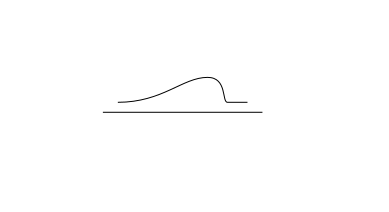
\includegraphics{figures/fig61-5.4.eps}
\caption{}
\label{chap1:fig5.4}
\end{figure}\pageoriginale

Carrier and Greenspan \cite{key4} give other solutions and include the anslysis for solving the general initial value problem.

\section{Bore on beach}\label{chap5:sec5.5}

When breaking occurs, a discontinuous ``bore'', corresponding to the shocks discussed earlier would be fitted in. The appropriate jump conditions were noted in Section \ref{chap4:sec4.1}. This has not been carried through in the Carrier-Greenspan solutions. However the simpler problem of what happens when a bore initially moving with constant speed and strength in an offshore region of constant depth impinges on a sloping beach has been studied by approximate and numerical methods. Reference may be made to the original papers \cite{key7} and \cite{key8} and recent additions in \cite{key9}.

\section{Edge waves}\label{chap5:sec5.6}

In the previous section we have considered only normal incidence with dependence only on distance $x$ normal to the shore. We now turn to phenomena that include longshore dependence. If $x_1$ is normal to and $x_2$ is along the shore, the linearized equation for the surface elevation $\eta(x_1,x_2,t)$ is modified from \eqref{chap5:eq5.10} to 
\begin{equation}
\eta_{tt}=g\beta x_1\left(\eta_{x_1 x_1}+\eta_{x_2 x_2}\right)+g\beta \eta_{x_1}. \tag{5.44}\label{chap5:eq5.44}
\end{equation}

The\pageoriginale modification is slight and we do not give the derivation.

We use separation of variables and let
\begin{equation}
\eta=N(x_1)e^{\pm ikx_2\pm i\omega t}.\tag{5.45}\label{chap5:eq5.45}
\end{equation}

Then $N(x_1)$ satisfies
\begin{equation}
N''+\frac{1}{x_1}N'+\left(\frac{\omega^2}{g\beta x_1}-k^2\right)N=0. \tag{5.46}\label{chap5:eq5.46}
\end{equation}

The interval of interest is $0<x_1<\infty$. The origin $x_1=0$ is a regular singular point; one solution is analytic and the other has a logarithmic singularity. At $\infty$, the equation is roughly 
\begin{align}
&N''-k^2N\simeq 0,\tag{5.47}\label{chap5:eq5.47}\\
\intertext{with solutions}
&N\simeq e^{-kx_1},\;e^{kx_1}.\tag{5.48}\label{chap5:eq5.48}
\end{align}

In this case only the solutions bounded at both $x_1=0$ and appear to be of interest. We shall see that the solutions represent waves running along the beach, and no-one seems to have interpreted the logarithmic solution in any sense such as breaking. So we choose the analytic solution near $x_1=0$. Then, in general, this solution will be a linear combination of both $e^{-kx_1}$ and $e^{+kx_1}$ at $\infty$. For an acceptable physical solution the term in $e^{kx_1}$ should be absent. This is possible only for special values of $\omega^2/g\beta$. We have a singular eigenvalue problem. If we set 
\begin{equation}
N=e^{-kx_1} F(X),\;X=2kx_1,\;k>0,\tag{5.49}\label{chap5:eq5.49}
\end{equation}
it becomes a standard one. We have 
\begin{equation}
XF_{XX}+(1-X)F_X+\frac{1}{2}\left(\frac{\omega^2}{g\beta k}-1\right)F=0, \tag{5.50}\label{chap5:eq5.50}
\end{equation}
and the required solutions are Laguerre polynomials
$$
L_n(X)=e^X\frac{d^n}{dx^n}\left(X^ne^{-X}\right),
$$\pageoriginale
with
\begin{equation}
\omega^2=gk(2n+1)\beta, \;n=\text{positive integer} \tag{5.51}\label{chap5:eq5.51}
\end{equation}

The solution for $N(x_1)$ is 
\begin{equation}
N(x_1)=e^{-kx_1}L_n(2kx_1).\tag{5.52}\label{chap5:eq5.52}
\end{equation}

The final solutions for $\eta$ are 
\begin{equation}
\eta=e^{-|k|x_1}L_n\left(2|k|x_1\right)e^{\pm ikx_2\pm i\omega t}, \tag{5.53}\label{chap5:eq5.53}
\end{equation}
where $|k|$ is appropriate if negative values of $k$ are used. 

These solutions all decay away from the shoreline and have crests perpendicular to the shoreline. For this reason they are known as `edge waves'. The lowest mode $n=0$ has 
$$
N(x_1)=e^{-kx_1},\;\omega^2=gk\beta,\;k>0,
$$
and one might take for example
\begin{equation}
\eta=e^{-kx_1}\cos\left(kx_2-\omega t\right).\tag{5.54}\label{chap5:eq5.54}
\end{equation}

This corresponds to a solution first found by Stokes. It is interesting to note how the different terms in \eqref{chap5:eq5.54} are balanced by this solution. One might note the propagation speed is $\sqrt{g\beta x_1}$ and expect the waves to swing round to the beach due to the increase of speed with $x_1$. The final result avoids this and we see from \eqref{chap5:eq5.54} that the balance is 
\begin{equation}
\eta_{x_1x_1}+\eta_{x_2x_2}=0,\;\eta_{tt}=g\beta\eta_{x_1} \tag{5.55}\label{chap5:eq5.55}
\end{equation}

The propagation speed argument applies directly when $\eta_{tt}$ balances the second derivatives in $(x_1,x_2)$; the balance in \eqref{chap5:eq5.55} avoids this.

The\pageoriginale equation is hyperbolic but these particular solutions avoid the hyperbolic character and appear as `dispersive waves' with dispersion relations given in \eqref{chap5:eq5.51}. (See \cite{key1} Chapter 1 for a discussion of the distinctions, and Chapter 11 for the main properties of dispersive waves).

We also note there is no possibility of an oblique wave at $\infty$. This would require
$$
\eta\sim e^{\pm i\ell x_1\pm ikx_2\pm i\omega t}
$$
with real $\ell$ and $k$. We have only the wave of normal incidence found in Section \ref{chap5:sec5.5},
\begin{equation}
\eta=J_0\left(2\omega \sqrt{\frac{x}{g\beta}}\right)e^{\pm i\omega t}, \tag{5.56}\label{chap5:eq5.56}
\end{equation}
or the edge waves travelling along the beach. As noted earlier, \eqref{chap5:eq5.56} does not have a finite nonzero amplitude at $\infty$, but it does at least represent a normal wave. For the oblique case there is not even a corresponding solution. This again is a breakdown of the shallow water assumption in deep water. We can interpret the result roughly by remarking that oblique deep water waves would in reality swing around towards the shore when they feel the depth decrease. They do this completely, and achieve normal incidence as in \eqref{chap5:eq5.56}, by the time the shallow water theory applies. In the linear theory, edge waves are not stimulated directly by incoming waves at infinity. We check these explanations from the full linear theory in Chapter \ref{chap7}. 

\section{Initial value problem and completeness}\label{chap5:sec5.7}\pageoriginale

Conversely if we turn to the case of an initial disturbance of finite extent, we need only the edge waves. The solutions \eqref{chap5:eq5.52} for integers $n\geq 0$ form a complete set, and any square integrable function of $x_1$ can be represented as an infinite series. Combined with a Fourier integral with respect to $x_2$ in \eqref{chap5:eq5.53}, we can represent any square integrable function of $(x_1,x_2)$. For example, the solution of the initial value problem
$$
\eta=\eta_0\left(x_1,x_2\right),\;\eta_t=0,\quad\text{at}\quad t=0
$$
would be 
\begin{equation}
\eta=\sum\limits_{m=0}^\infty\int\limits_{-\infty}^\infty A_m(k)e^{-|k|x_1}L_m\left(2 |k|x_1\right)e^{ikx_2}\cos t\sqrt{g(2m+1)|k|}\,dk,\tag{5.57}\label{chap5:eq5.57}
\end{equation}
where, using the two inversion formulas,
\begin{equation}
A_m(k)=\frac{1}{\pi}\int\limits_0^\infty \int\limits_{-\infty}^\infty\eta_0\left( \xi_1,\xi_2\right)e^{-|k|\xi_1}L_m\left(2|k|\xi_1\right)\frac{|k|}{(m!)^2} e^{-ik\xi_2}\,d\xi_1\,d\xi_2.\tag{5.58}\label{chap5:eq5.58}
\end{equation}

A term proportional to \eqref{chap5:eq5.56} is not required since the Laguerre polynomials are already complete. Of course, one would expect the solution for an initial disturbance that is very long in the $x_2$ direction to be represented closely by a superposition of the normal incidence solutions \eqref{chap5:eq5.56}. To resolve the apparent difference in form, we consider the case
$$
\eta_0\left(x_1,x_2\right)=f(x_1)g(x_2);
$$
then
$$
A_m(k)=\int\limits_0^\infty f(\xi_1)e^{-|k|\xi_1}L_m\left(2|k|\xi_1\right) \frac{2|k|}{(m!)^2}\,d\xi_1\times\frac{1}{2\pi}\int\limits_{-\infty}^\infty g(\xi_2)e^{-ik\xi_2}\,d\xi_2.
$$\pageoriginale

As $g\to 1$, the second factor in $A_m(k)$ becomes the Dirac delta function $\delta(k)$. Hence, after substitution in \eqref{chap5:eq5.57} we have 
{\fontsize{10}{12}\selectfont
$$
\eta=\underset{k\to 0}{\lim}\left\{\sum\limits_{m=0}^\infty
\left(\int\limits_0^\infty\frac{f(\xi_1)L_m\left(2|k|\xi_1\right)\,d\xi_1}{m!}
\,\frac{L_m\left(2|k|x_1\right)}{m!}\cos\sqrt{g|k|(2m+1)}t.2|k|\right.\right\}. 
$$} 

Because of the factor $|k|$, the contribution comes from the additon of many small terms for large $m$. As $m\to\infty, |k|m$ finite,
\begin{equation}
\frac{L_m\left(2|k|x_1\right)}{m!}\sim J_0\left(2\sqrt{2m|k|x_1}\right). \tag{5.59}\label{chap5:eq5.59}
\end{equation}

Using this and introducing 
$$
-\frac{\omega_m^2}{g\beta}=2|k|m,\; 2|k|-\Delta\left(\frac{\omega_m^2}{g\beta} \right),
$$
we have 
{\fontsize{10}{12}\selectfont
$$
\eta\sim\sum\limits_{m=0}^\infty\left\{\int\limits_0^\infty
f(\xi_1)J_0 \left(2 \omega_m
\sqrt{\frac{\xi_1}{g\beta}}\right)\,d\xi_1\right\}\times J_0\left(2
\omega_m \sqrt{\frac{x_1}{g\beta}}\right)\cos\omega_m t.\Delta\left(
\frac{\omega_m^2}{g\beta}\right). 
$$}

This is the Riemann sum for 
$$
\eta=\int\limits_0^\infty\left\{\int\limits_0^\infty f(\xi_1)J_0\left(2\omega \sqrt{\frac{\xi_1}{g\beta}} \; \right)\,d\xi_1\right\}J_0\left(2\omega \sqrt{\frac{x_1}{g\beta}} \; \right)\cos \omega t\Delta\left(\frac{\omega^2} {g\beta}\right).
$$

This is the result for $\eta_0(x_1)=f(x_1)$ using the Fourier-Bessel expansion with \eqref{chap5:eq5.56}. The key relation to the correspondence is of course the approximation \eqref{chap5:eq5.59}.

\section{Weather fronts}\label{chap5:sec5.8}\pageoriginale 

In the atmosphere when a layer of cold air pushes under a layer of warmer air, a wedge shaped region of cold air is often formed; it is controlled by the Coriolis forces. Disturbances running along the front of this wedge have important meteorological effects. In an ideal situation (the formulation of approximate equations given in Stoker \cite{key10}, Chapter 10.11), these are like the above edge waves, and the analysis in Laguerre polynomials is similar. This gives further stimulation for the interest in this kind of wedge problem.

